%!TeX spellcheck = el_GR-en_US
%!TEX TS-program = xelatex

\documentclass{mycv}

\RequirePackage[greek]{datetime2} 		 % show greek date correctly using \today command
\renewcommand{\today}{\ifcase\month\or
	Ιανουάριος\or Φεβρουάριος\or Μάρτιος\or% 
	Απρίλιος\or Μάιος\or Ιούνιος\or Ιούλιος%
	\or Αύγουστος\or Σεπτέμβριος\or% 
	Οκτώβριος\or Νοέμβριος\or% 
	Δεκέμβριος\fi\ \number \year}			 % nominative instead of genitive 
\RequirePackage{amsmath}

\hypersetup{%
	pdftitle={Άγγελος Αρεκλάκης - Βιογραφικό Σημείωμα},
	pdfauthor={Άγγελος Αρεκλάκης},
	pdfsubject={Βιογραφικό Σημείωμα},
	pdfkeywords={Άγγελος Αρεκλάκης,Βιογραφικό Σημείωμα,CV},
	pdflang={el-GR}
}

\begin{document}
	\pagestyle{empty}
	\begin{minipage}{.7\textwidth}
		\begin{flushleft}
			\name{Άγγελος Αρεκλάκης}{Μηχανικός Λογισμικού}{Systems Administrator}
			\contact{+30 6978406795}{angelosareklis@outlook.com}
			\centering
			{\bf Ημερομηνία Γέννησης}: 18 Σεπτεμβρίου 1994  {\Large\textperiodcentered} {\bf Τοποθεσία}: Θεσσαλονίκη, Ελλάδα
		\end{flushleft}
	\end{minipage}
	\begin{minipage}{.3\textwidth}
		\begin{flushright}
			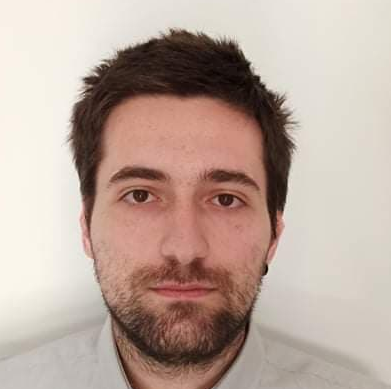
\includegraphics[scale=0.3]{assets/angelos.png}
		\end{flushright}
	\end{minipage}
	%
	\vspace*{-0.5cm}
	%
	\section{Εισαγωγικό Σημείωμα}
	\textnormal Το όνομά μου είναι Άγγελος Αρεκλάκης. Είμαι τελειόφοιτος του τμήματος Ηλεκτρολόγων Μηχανικών και Μηχανικών Υπολογιστών του Πανεπιστημίου Δυτικής Μακεδονίας. Γεννήθηκα το 1994 στην Ξάνθη αλλα μεγάλωσα στην Θεσσαλονίκη.Το 2021 τελείωσα με τις στρατιωτικές μου υποχρεώσεις. Μιλάω εξαιρετικά καλά Αγγλικά και καλά Γαλλικά . Πάθος μου είναι η επίλυση προβλημάτων και ο σχεδιασμός λύσεων. Προσπαθώ να μαθαίνω συνεχώς περισσότερα και να αποκτώ δεξιότητες, χρησιμοποιώντας τα πιο ενημερωμένα εργαλεία. 

	\section{Εμπειρία}

	\begin{EntryDated}{Ελεύθερος Επαγγελματίας}{}{2018 -- Τώρα}{Προγραμματιστής}{-1cm}
	\begin{Itemize}
		\item Εργασίες ανάπτυξης λογισμικού και ιστοσελίδων, για ιδιώτες και επιχειρήσεις.
	\end{Itemize}
	\end{EntryDated}

	\section{Δεξιότητες}
	\begin{tabular}{m{4.5cm} m{13cm}}
		\textbf{Διάγνωση / Επιδιόρθωση}     & Διάγνωση και επίλυση προβλημάτων υλικού και λογισμικού. \\
		\textbf{Διαχείριση Συστημάτων}		& Unix, NGINX, VMware/Virtualbox \\
		\textbf{Προγραμματισμός} 	 	  	& C/C++, Java, \LaTeX \\
		\textbf{Προγρ. Διαδικτύου}	  		& HTML/CSS, Bootstrap, Javascript, JQuery, Ajax, PHP, SQL, Wordpress \\
		\textbf{Λειτουργικά Συστήματα}   	& Windows \\
		\textbf{Διάφορα}        		 	& Σουίτες Office, Αλγοριθμική Σχεδίαση, Οργάνωση Project, Άδεια Οδήγησης Κατηγορίας Β \\
		\textbf{Γλώσσες} 			   		& Ελληνικά (μητρική γλώσσα), Αγγλικά, Γαλλικά
	\end{tabular}

	\section{Εκπαίδευση}

	\begin{EntryDatedLogo}{Πανεπιστήμιο Δυτικής Μακεδονίας}{https://ece.uowm.gr}{2014 -- Τώρα}{Τμήμα Ηλεκτρολόγων Μηχανικών και Μηχανικών Υπολογιστών}{-0.3cm}{assets/uowm.pdf}{0.6}
	\begin{Itemize}
		\item Απομένει η εκπόνηση της διπλωματικής μου εργασίας για την ολοκλήρωση των σπουδών μου.
	\end{Itemize}
	\end{EntryDatedLogo}

	\section{Εθελοντική Εργασία}
	\begin{EntryDatedLogo}{Κέντρο Κοινωνικής Πρόνοιας Κεντρικής Μακεδονίας}{http://www.kkp-km.gr/}{2018 -- 2019}{Ανάπτυξη Λογισμικού}{-0.3cm}{assets/kkpkm.pdf}{0.75}
		\begin{Itemize}
			\item developer και σχεδιαστής ενός web application που καταγράφει και διαχειρίζεται τις θεραπείες των περιθαλπόμενων ενός ιδρύματος.
			\item Περισσότερες πληροφορείες στο site του  \href{https://diavgeia.gov.gr/decision/view/\%CE\%A8\%CE\%A6\%CE\%A1\%CE\%93\%CE\%9F\%CE\%9E\%CE\%A7\%CE\%A3-\%CE\%A0\%CE\%93\%CE\%A6}{\textit{diavgeia}}.
		\end{Itemize}
	\end{EntryDatedLogo}

\end{document}